\documentclass[namecite, fleqn]{goose-article}

\title{Non-linear elasticity}

\author{Tom W.J.\ de Geus}

\hypersetup{pdfauthor={T.W.J. de Geus}}

\begin{document}

\maketitle

\begin{abstract}
This constitutive model encompasses a non-linear, but history independent,
relation between the Cauchy stress, $\bm{\sigma}$,
and the linear strain tensor, $\bm{\varepsilon}$, i.e.:
\begin{equation*}
    \bm{\sigma} = f \left( \bm{\varepsilon} \right)
\end{equation*}
The model is implemented in 3-D, hence it can directly be used for either 3-D or
2-D plane strain problems.
\end{abstract}

\section{Constitutive model}

The following strain-energy is defined:
\begin{equation}
    U ( \bm{\varepsilon} )
    = \frac{9}{2} K \varepsilon_\mathrm{m}
    + \frac{ \sigma_0 \, \varepsilon_0 }{ n+1 }
    \left( \frac{\varepsilon_\mathrm{eq}}{\mathrm{\varepsilon_0}} \right)^{n+1}
\end{equation}
where $K$ is the bulk modulus, $\varepsilon_0$ and $\sigma_0$ are a reference strain and
stress respectively, and $n$ is an exponent that sets the degree of non-linearity.
Finally $\varepsilon_\mathrm{m}$ and $\varepsilon_\mathrm{eq}$ are the hydrostatic and
equivalent strains (see \cref{sec:ap:strain}).

This leads to the following stress--strain relation:
\begin{equation}
\label{eq:stress}
    \bm{\sigma}
    = \frac{\partial U}{\partial \bm{\varepsilon}}
    = 3 K \varepsilon_\mathrm{m} \, \bm{I}
    + \frac{2}{3} \frac{\sigma_0}{\varepsilon_0^n} \,
    \varepsilon_\mathrm{eq}^{n-1} \, \bm{\varepsilon}_\mathrm{d}
\end{equation}
see \cref{sec:ap:nomenclature} for nomenclature.

\section{Consistent tangent}

The consistent tangent maps a variation in strain, $\delta \bm{\varepsilon}$,
to a variation in stress, $\delta \bm{\sigma}$, as follows
\begin{equation}
  \delta \bm{\sigma} = \mathbb{C} : \delta \bm{\varepsilon}
\end{equation}
The tangent, $\mathbb{C}$, thus corresponds to the derivative of \cref{eq:stress} w.r.t.\ strain.
For this, the chain rule is employed:
\begin{equation}
    \mathbb{C}
    = \frac{\partial}{\partial \bm{\varepsilon}}
    \bigg[\;
        3 K \varepsilon_\mathrm{m} \, \bm{I}
    \;\bigg]
    + \frac{\partial}{\partial \bm{\varepsilon}_\mathrm{d}}
    \bigg[\;
        \frac{2}{3} \frac{\sigma_0}{\varepsilon_0^n} \,
        \varepsilon_\mathrm{eq}^{n-1} \, \bm{\varepsilon}_\mathrm{d}
    \;\bigg]
    : \frac{\partial \bm{\varepsilon}_\mathrm{d}}{\partial \bm{\varepsilon}}
\end{equation}
Where:
\begin{itemize}

    \item the derivative of the volumetric part reads
    \begin{equation}
        \frac{\partial}{\partial \bm{\varepsilon}}
        \bigg[\;
            3 K \varepsilon_\mathrm{m} \, \bm{I}
        \;\bigg]
        = K \bm{I} \otimes \bm{I}
    \end{equation}

    \item the chain rule for the deviatoric part reads
    \begin{align}
        \frac{\partial}{\partial \bm{\varepsilon}_\mathrm{d}}
        \bigg[\;
            \varepsilon_\mathrm{eq}^{n-1} \, \bm{\varepsilon}_\mathrm{d}
        \;\bigg]
        &=
        \frac{
            \partial \big[ \varepsilon_\mathrm{eq}^{n-1} \big]
        }{
            \partial \bm{\varepsilon}_\mathrm{d}
        } \otimes \bm{\varepsilon}_\mathrm{d}
        + \varepsilon_\mathrm{eq}^{n-1}
        \frac{
            \partial \bm{\varepsilon}_\mathrm{d}
        }{
            \partial \bm{\varepsilon}_\mathrm{d}
        }
        \\
        &=
        \tfrac{2}{3} (n-1) \, \varepsilon_\mathrm{eq}^{n-3} \,
        \bm{\varepsilon}_\mathrm{d} \otimes \bm{\varepsilon}_\mathrm{d}
        + \varepsilon_\mathrm{eq}^{n-1} \, \mathbb{I}
    \end{align}

    \item and it has been used that
    \begin{align}
        \frac{\partial}{\partial \bm{\varepsilon}_\mathrm{d}}
        \bigg[\;
            \varepsilon_\mathrm{eq}^{n-1}
        \;\bigg]
        &= (n-1)\, \varepsilon_\mathrm{eq}^{n-2} \,
        \frac{2}{3} \frac{\bm{\varepsilon}_\mathrm{d}}{\varepsilon_\mathrm{eq}}
        \\
        &= \tfrac{2}{3} (n-1) \,
        \varepsilon_\mathrm{eq}^{n-3} \, \bm{\varepsilon}_\mathrm{d}
    \end{align}

\end{itemize}

Combining the above yields:
\begin{align}
    \mathbb{C}
    &= K \bm{I} \otimes \bm{I} +
    \frac{2}{3} \frac{\sigma_0}{\varepsilon_0^n}
    \bigg(
        \tfrac{2}{3} (n-1) \, \varepsilon_\mathrm{eq}^{n-3}
        \bm{\varepsilon}_\mathrm{d} \otimes \bm{\varepsilon}_\mathrm{d}
        + \varepsilon_\mathrm{eq}^{n-1} \mathbb{I}
    \bigg) : \mathbb{I}_\mathrm{d} \\
    &= K \bm{I} \otimes \bm{I} +
    \frac{2}{3} \frac{\sigma_0}{\varepsilon_0^n}
    \bigg(
        \tfrac{2}{3} (n-1) \, \varepsilon_\mathrm{eq}^{n-3}
        \bm{\varepsilon}_\mathrm{d} \otimes \bm{\varepsilon}_\mathrm{d}
        + \varepsilon_\mathrm{eq}^{n-1} \, \mathbb{I}_\mathrm{d}
    \bigg)
\end{align}

\section{Consistency check}

To check if the derived tangent $\mathbb{C}$ a \emph{consistency check} can be performed.
A (random) perturbation $\delta \bm{\varepsilon}$ is applied.
The residual is compared to that predicted by the tangent.
For the general case of linearisation, the following holds:
\begin{equation}
    \bm{\sigma}\big( \bm{\varepsilon}_\star + \delta \bm{\varepsilon} \big) =
    \bm{\sigma}\big( \bm{\varepsilon}_\star \big) +
    \mathbb{C} \big( \bm{\varepsilon}_\star \big) : \delta \bm{\varepsilon} +
    \mathcal{O}(\delta \bm{\varepsilon}^2)
\end{equation}
or
\begin{equation}
    \underbrace{
        \bm{\sigma}\big( \bm{\varepsilon}_\star + \delta \bm{\varepsilon} \big) -
        \bm{\sigma}\big( \bm{\varepsilon}_\star \big)
    }_{
        \displaystyle \delta \bm{\sigma}
    } -
    \mathbb{C} \big( \bm{\varepsilon}_\star \big) : \delta \bm{\varepsilon} =
    \mathcal{O}(\delta \bm{\varepsilon}^2)
\end{equation}
This allows the introduction of a relative error
\begin{equation}
  \eta =
  \Big|\Big|
        \delta \bm{\sigma} -
        \mathbb{C}(\bm{\varepsilon}_\star) : \delta \bm{\varepsilon}
  \Big|\Big|
  /
  \Big|\Big| \delta \bm{\sigma} \Big|\Big|
\end{equation}
This \emph{truncation error} thus scales as $\eta \sim || \delta \bm{\varepsilon} ||^2$
as depicted in \cref{fig:consistency:expected}.
As soon as the error becomes sufficiently small the numerical \emph{rounding error}
becomes more dominant, the scaling thereof is also included in \cref{fig:consistency:expected}.

\begin{figure}[htp]
    \centering
    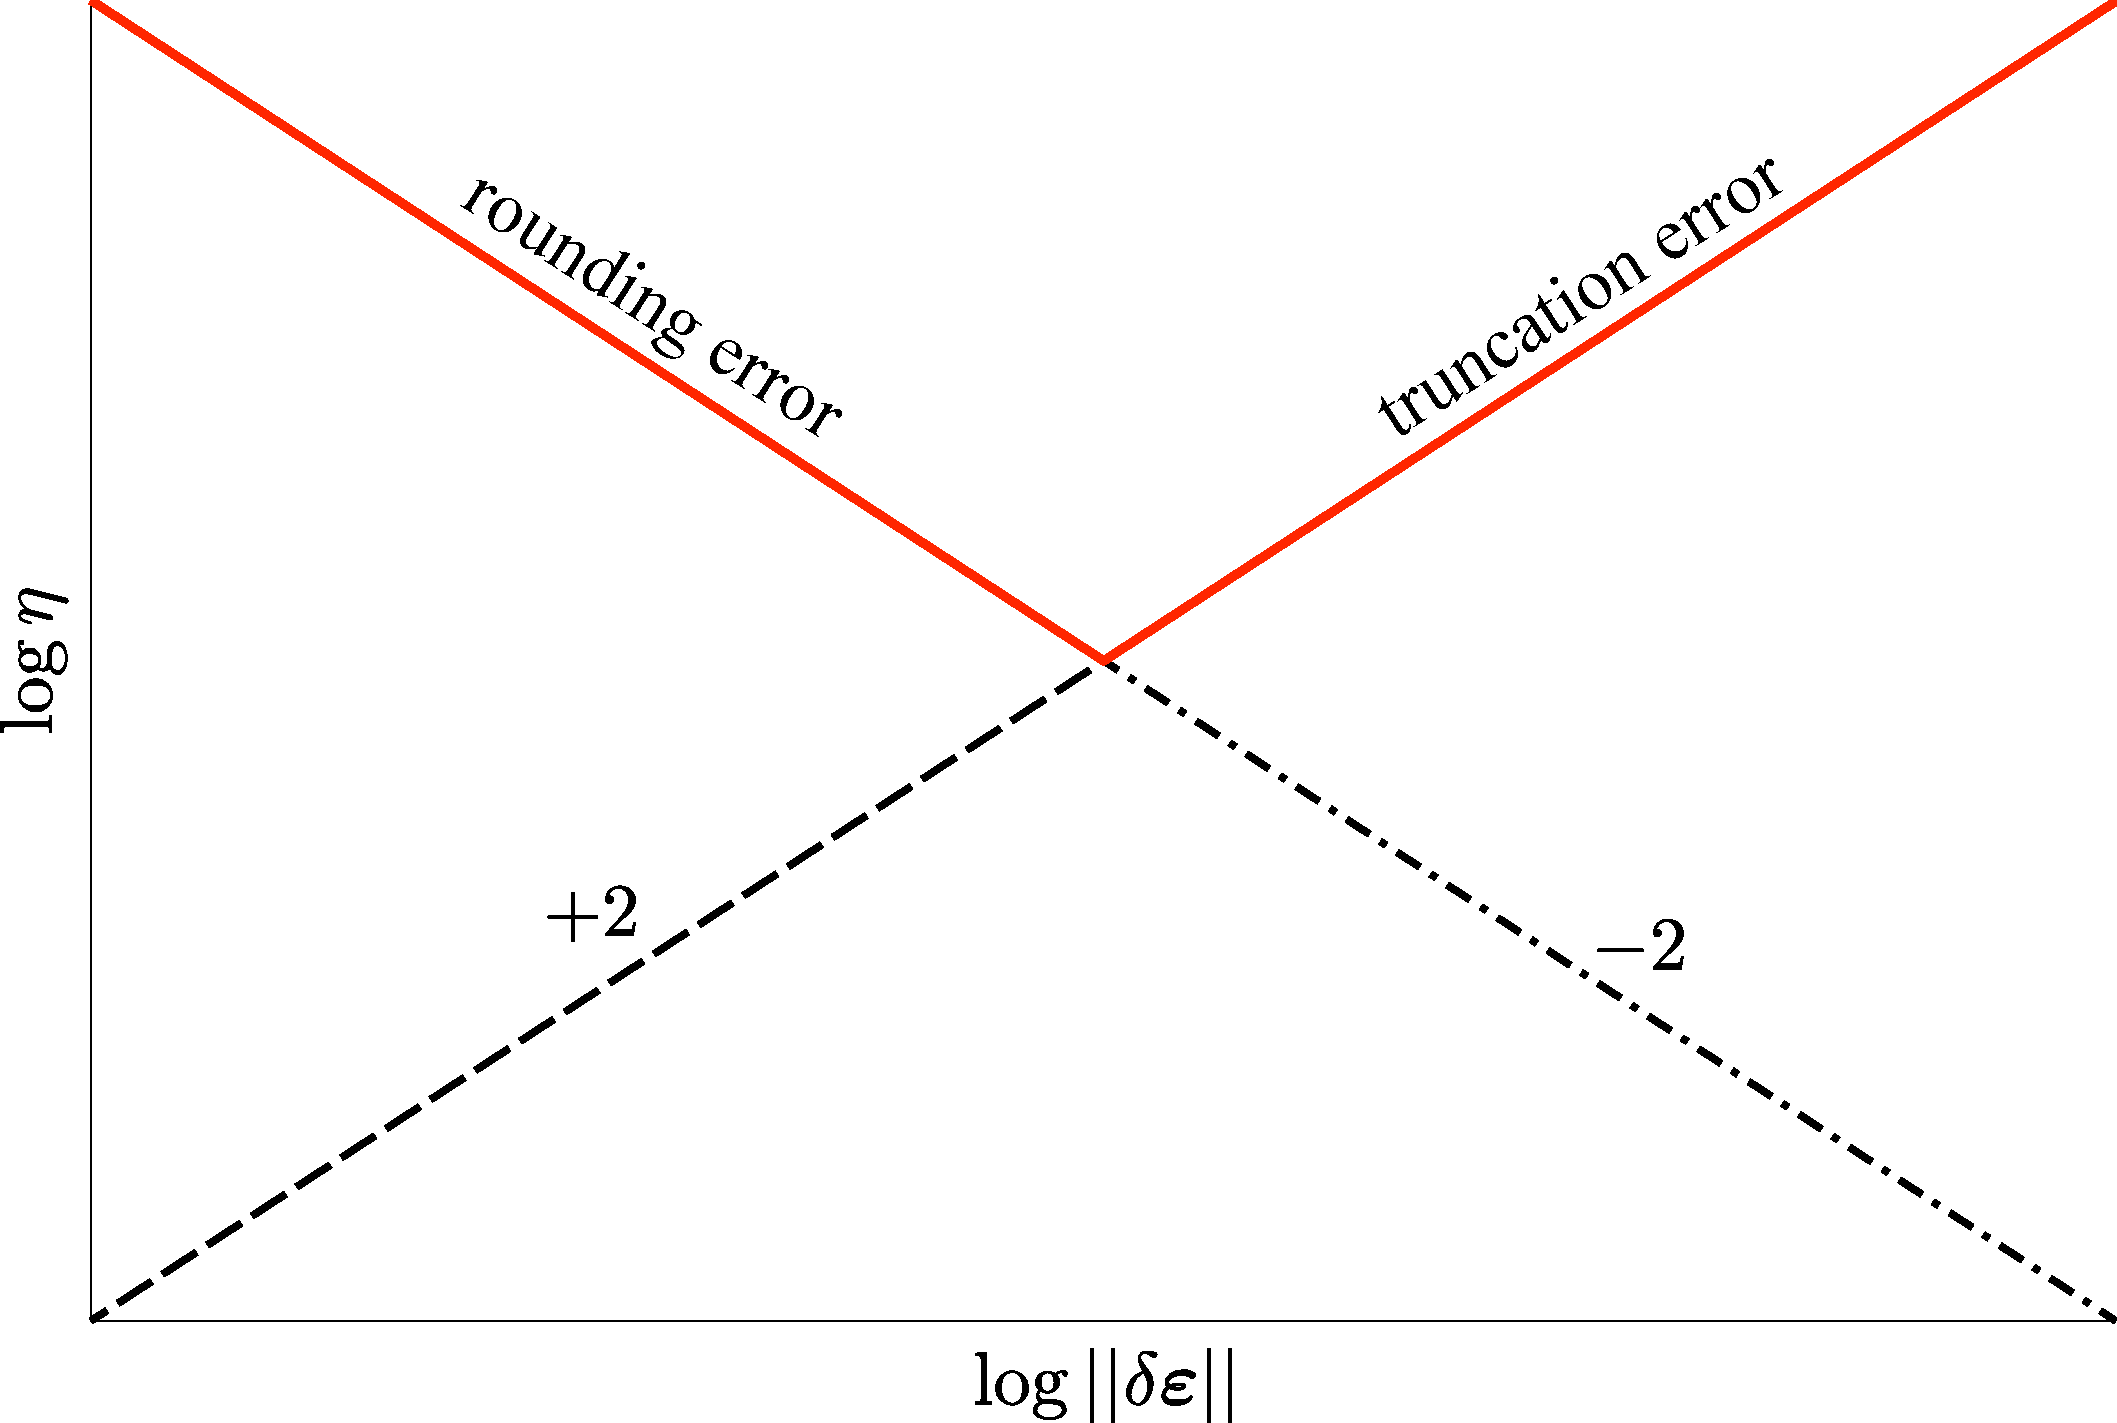
\includegraphics[width=.5\textwidth]{figures/consistency}
    \caption{Expected behaviour of the consistency check, see \citet[p.~9]{Heath2002}.}
    \label{fig:consistency:expected}
\end{figure}

The measurement of $\eta$ and a function of $|| \delta \bm{\varepsilon} ||$, as depicted in
\cref{fig:consistency}, indeed matches the prediction in \cref{fig:consistency:expected}.

\begin{figure}[htp]
    \centering
    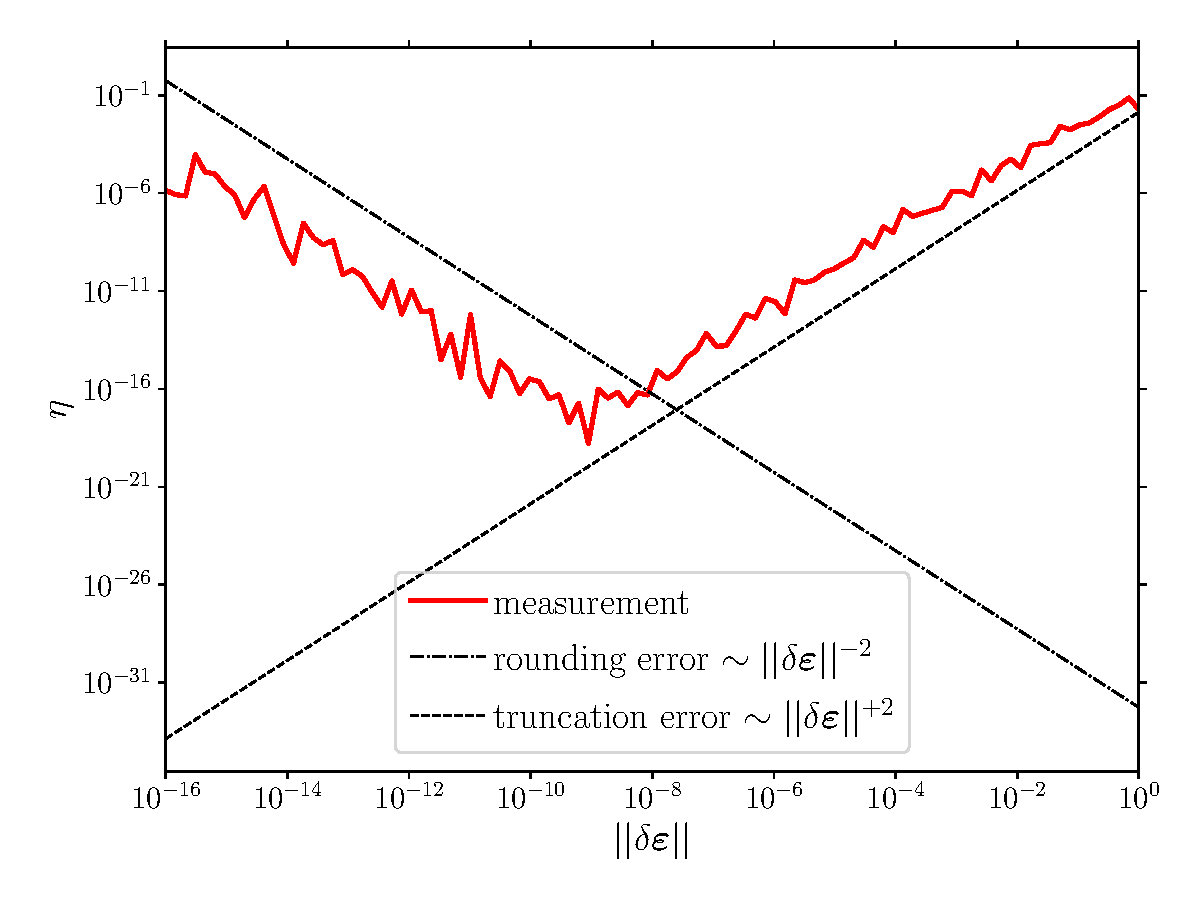
\includegraphics[width=.5\textwidth]{examples/consistency}
    \caption{Measured consistency check, cf.\ \cref{fig:consistency:expected}.}
    \label{fig:consistency}
\end{figure}

\bibliography{library}

\appendix
\vfill\newpage

\section{Nomenclature}
\label{sec:ap:nomenclature}

\paragraph{Tensor products}
\vspace*{.5eM}

\begin{itemize}

    \item Dyadic tensor product
    \begin{align}
        \mathbb{C} &= \bm{A} \otimes \bm{B} \\
        C_{ijkl} &= A_{ij} \, B_{kl}
    \end{align}

    \item Double tensor contraction
    \begin{align}
        C &= \bm{A} : \bm{B} \\
        &= A_{ij} \, B_{ji}
    \end{align}

\end{itemize}

\paragraph{Tensor decomposition}
\vspace*{.5eM}

\begin{itemize}

    \item Deviatoric part $\bm{A}_\mathrm{d}$ of an arbitrary tensor $\bm{A}$:
    \begin{equation}
        \mathrm{tr}\left( \bm{A}_\mathrm{d} \right) \equiv 0
    \end{equation}
    and thus
    \begin{equation}
        \bm{A}_\mathrm{d} = \bm{A} - \tfrac{1}{3} \mathrm{tr}\left( \bm{A} \right)
    \end{equation}

\end{itemize}

\paragraph{Fourth order unit tensors}
\vspace*{.5eM}

\begin{itemize}

    \item Unit tensor:
    \begin{equation}
        \bm{A} \equiv \mathbb{I} : \bm{A}
    \end{equation}
    and thus
    \begin{equation}
        \mathbb{I} = \delta_{il} \delta{jk}
    \end{equation}
    \item Right-transposition tensor:
    \begin{equation}
        \bm{A}^T \equiv \mathbb{I}^{RT} : \bm{A} = \bm{A} : \mathbb{I}^{RT}
    \end{equation}
    and thus
    \begin{equation}
        \mathbb{I}^{RT} = \delta_{ik} \delta_{jl}
    \end{equation}
    \item Symmetrisation tensor:
    \begin{equation}
        \mathrm{sym} \left( \bm{A} \right) \equiv \mathbb{I}_\mathrm{s} : \bm{A}
    \end{equation}
    whereby
    \begin{equation}
        \mathbb{I}_\mathrm{s} = \tfrac{1}{2} \left( \mathbb{I} + \mathbb{I}^{RT} \right)
    \end{equation}
    This follows from the following derivation:
    \begin{align}
        \mathrm{sym} \left( \bm{A} \right) &= \tfrac{1}{2} \left( \bm{A} + \bm{A}^T \right)
        \\
        &= \tfrac{1}{2} \left( \mathbb{I} : \bm{A} + \mathbb{I}^{RT} : \bm{A} \right)
        \\
        &= \tfrac{1}{2} \left( \mathbb{I} + \mathbb{I}^{RT} \right) : \bm{A}
        \\
        &= \mathbb{I}_\mathrm{s} : \bm{A}
    \end{align}

    \item Deviatoric and symmetric projection tensor
    \begin{equation}
        \mathrm{dev} \left( \mathrm{sym}
        \left( \bm{A} \right) \right) \equiv \mathbb{I}_\mathrm{d} : \bm{A}
    \end{equation}
    from which it follows that:
    \begin{equation}
        \mathbb{I}_\mathrm{d}
        = \mathbb{I}_\mathrm{s} - \tfrac{1}{3} \bm{I} \otimes \bm{I}
    \end{equation}

\end{itemize}

\section{Strain measures}
\label{sec:ap:strain}

\begin{itemize}

    \item Mean strain
    \begin{equation}
        \varepsilon_\mathrm{m}
        = \tfrac{1}{3} \, \mathrm{tr} ( \bm{\varepsilon} )
        = \tfrac{1}{3} \, \bm{\varepsilon} : \bm{I}
    \end{equation}
    \item Strain deviator
    \begin{equation}
        \bm{\varepsilon}_\mathrm{d}
        = \bm{\varepsilon} - \varepsilon_\mathrm{m} \, \bm{I}
        = \mathbb{I}_\mathrm{d} : \bm{\varepsilon}
    \end{equation}
    \item Equivalent strain
    \begin{equation}
        \varepsilon_\mathrm{eq}
        = \; \sqrt{
            \tfrac{2}{3} \, \bm{\varepsilon}_\mathrm{d} : \bm{\varepsilon}_\mathrm{d}
        }
    \end{equation}

\end{itemize}

\section{Variations}
\label{sec:ap:variations}

\begin{itemize}

    \item Strain deviator
    \begin{equation}
        \delta \bm{\varepsilon}_\mathrm{d}
        = \left( \mathbb{I}_\mathrm{s} - \tfrac{1}{3} \bm{I} \otimes \bm{I} \right) :
        \delta \bm{\varepsilon}
        = \mathbb{I}_\mathrm{d} : \delta \bm{\varepsilon}
    \end{equation}

    \item Mean equivalent strain
    \begin{equation}
        \delta \varepsilon_\mathrm{m}
        = \tfrac{1}{3} \bm{I} : \delta \bm{\varepsilon}
    \end{equation}

    \item Von Mises equivalent strain
    \begin{align}
        \delta \varepsilon_\mathrm{eq}
        &= \frac{1}{3} \frac{1}{\varepsilon_\mathrm{eq}}
        \left( \bm{\varepsilon}_\mathrm{d} : \delta \bm{\varepsilon}_\mathrm{d} +
        \delta \bm{\varepsilon}_\mathrm{d} : \bm{\varepsilon}_\mathrm{d} \right) \\
        &= \frac{2}{3} \frac{1}{\varepsilon_\mathrm{eq}}
        \left( \bm{\varepsilon}_\mathrm{d} : \delta \bm{\varepsilon}_\mathrm{d} \right) \\
        &= \frac{2}{3} \frac{\bm{\varepsilon}_\mathrm{d}}{\varepsilon_\mathrm{eq}} :
        \delta \bm{\varepsilon}_\mathrm{d}
    \end{align}

\end{itemize}

\end{document}
